\begin{exercise}{Spectromètre de masse}{2}{Sup}
{Particuleschargees}{lelay}

On s'intéresse au spectromètre de masse, un dispositif permettant de discriminer des ions par rapport à leur rapport masse sur charge $\mu$.

\begin{multicols}{2}
\begin{figure}[H]
    \centering
    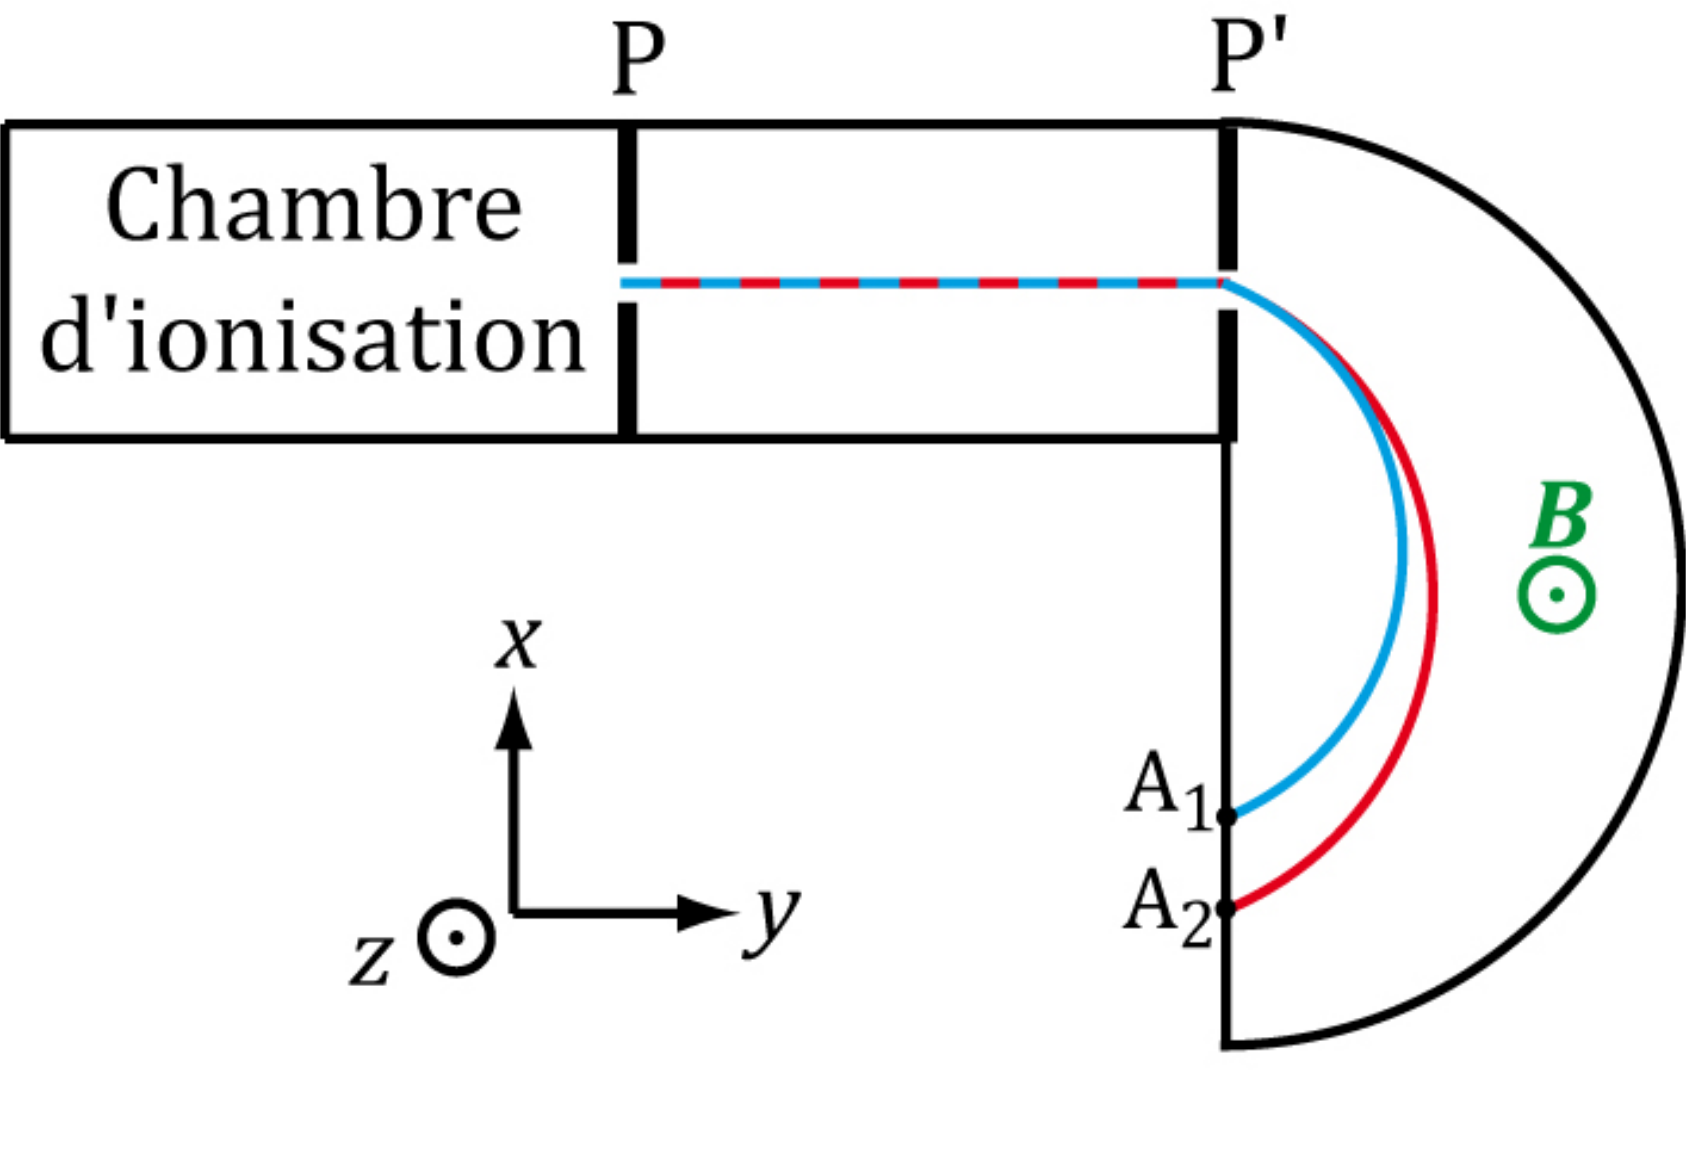
\includegraphics[width=.8\linewidth]{meca/particuleschargees/spectromasse.png}
    \caption{Schéma simplifié d'un spectromètre de masse.}
\end{figure}
\begin{figure}[H]
    \centering
    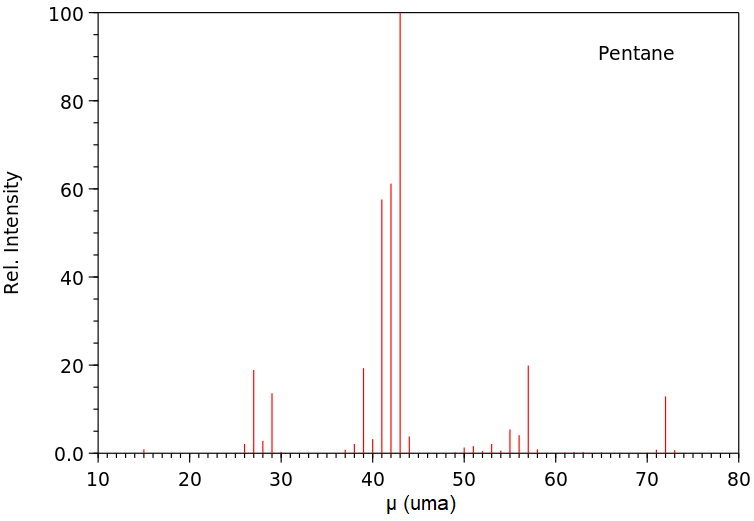
\includegraphics[width=\linewidth]{meca/particuleschargees/mass_pentane.png}
    \caption{Spectre de masse du pentane.}
\end{figure}
\end{multicols}

Le principe est schématisé en figure 1. Dans la chambre d'ionisation on transforme les molécules en ions de faible vitesse. Ils passent ensuite dans un accélérateur linéaire où une tension $U = 8$ kV est imposée entre les plaques $P$ et $P'$. Enfin ils sont soumis dans la zone de déviation à un champ $\vec{B} = B_0\vec{e}_z$, avec $B_0 = 4$ T.

\begin{questions}
    \questioncours Force de Lorentz
    \question On considère deux particules de masse $m_1$ et $m_2$ et de charge $q_1$ et $q_2$. Donner leur vitesse respectives $v_1$ et $v_2$ en sortie de la zone d'accélération. On introduira $\mu = m e/q$, le rapport de masse (sur charge).
    \question Décrire la trajectoire des ions dans la zone de déviation. Quels sont les rayons $R_1$ et $R_2$ de ces trajectoires ?
    \question En déduire l'exrepssion de la distance $d = A_1A_2$ séparant les points d'impact des ions sur la plaque finale en fonction des rapport de masse $\mu_1$ et $\mu_2$. Pourquoi accélère-t-on les ions avant qu'ils entrent dans la zone de déviation ?
    \question Quel est le rapport de masse d'un ion éthyle (chargé +1) dans le SI et en uma ? En ordre de grandeur, calculer la distance nécessaire pour résoudre des écarts de masse de l'ordre d'un nucléon (de 1 uma) sur l'ion méthyle.
    \question On donne le spectre de masse du pentane en figure 2. En quels ions le pentane est susceptible de se fractionner ? Quels sont leur $\mu$ ? Interpréter le spectre.
\end{questions}

\paragraph{Données :}
\begin{itemize}
    \item unité de masse atomique : $1$ uma $= 1,66\times 10^{-27}$ kg ;
    \item masse d'un atome hydrogène : 1 uma, \quad masse d'un atome de carbone : 12 uma ;
    \item charge de l'électron $1,61 \times 10^{-19}$ C.
\end{itemize}
Dans la littérature, $\mu$ est plus souvent noté $m/z$.
\end{exercise}

\begin{solution}
    \begin{questions}
        \questioncours $\vF_\textsc{l} = q\vE + q\vv\wedge\vB$
        \question $\dfrac{1}{2}m v^2 = q U$ donc $v = \sqrt{\dfrac{2Ue}{\mu}}$.
        \question $m\dv{\vv}{t} = q\vv\wedge\vB$ d'ou $\omega_\text{c} = \dfrac{e B_0}{\mu}$ et $R = \dfrac{v \mu}{e B_0} = \sqrt{\dfrac{2U}{e B_0^2}} \sqrt{\mu}$.
        \question $d = \sqrt{\dfrac{2U}{e B_0^2}} (\sqrt{\mu_1} - \sqrt{\mu_2})$.
        \question Ethyle $\mathrm{C_2H_4^+}$ : $m = 28$ uma, $q = e$, $\mu = 28$ uma.
        Donc $d =  \sqrt{\dfrac{2U m_u}{e B_0^2}}(\sqrt{29} - \sqrt{28}) = 130$ $\mu$m.
        \question Typiquement le pentane se fragmente en :
        \begin{align*}
            \mathrm{C_5H_{12}} & \mathrm{\longrightarrow C_5H_{12}^+ \text{\small ($\mu = 72$)} + e^-} \\
            \mathrm{C_5H_{12}} & \mathrm{\longrightarrow C_4H_9^+ \text{\small ($\mu = 57$)} + CH_3^\bullet + e^-} \\
            \mathrm{C_5H_{12}} & \mathrm{\longrightarrow C_3H_7^+ \text{\small ($\mu = 43$)} + C_2H_5^\bullet + e^-} \\
            \mathrm{C_5H_{12}} & \mathrm{\longrightarrow C_2H_5^+ \text{\small ($\mu = 29$)} + C_3H_7^\bullet + e^-} \\
            \mathrm{C_5H_{12}} & \mathrm{\longrightarrow CH_3^+ + \text{\small ($\mu = 15$, non résolu)} + C_4H_9^\bullet + e^-}
        \end{align*}
        Les petits pics off de 1 ou 2 par rapport aux grands sont liés à des pertes d'un H typiquement.
    \end{questions}
\end{solution}